\section{From Gaussian pairs to energy comparisons}
\label{sec:energy}

The preceding sections construct the Fourier pair in
Theorem~\ref{thm:normalized-pair}.  We now turn that pair into a sharp energy
bound for every Gaussian.  Two steps are needed.  First, Fourier nonnegativity
gives a lower bound for any locally finite configuration with the stated
centered density.  Second, scaling and Fourier complementation turn the
normalized pair into a minorant for every positive Gaussian parameter.
Section~\ref{sec:mixtures} then completes the universal-energy theorem by
positive mixtures. The renormalized and jellium consequences are treated
separately in Section~\ref{sec:renormalized}.

\subsection{An area comparison under centered density}

Recall that $B_R$ is the centered closed disk,
$\mathcal C_R=\mathcal C\cap B_R$, and $N_R=\#\mathcal C_R$.
The only geometric limit used below is $N_R/(\pi R^2)\to1$.
The density-only linear-programming argument is due to
Cohn and de~Courcy-Ireland~\citep[Proposition~2.2]{CohnDeCourcyIreland2018}, whose background-measure
comparison follows Cohn and Zhao~\citep[Theorem~3.3]{CohnZhao2014}.  The latter is a packing
theorem; its exclusion-distance hypothesis is not an assumption here.
We give the argument for the exact auxiliary class used in this paper.

\begin{proposition}[Linear programming with centered disk density]
\label{prop:density-lp}
Let $f$ be a real even Schwartz function on $\R^2$ whose Fourier transform is
nonnegative.  Every locally finite configuration $\mathcal C\subset\R^2$
with centered disk density one satisfies
\begin{equation}\label{eq:density-lp}
 \liminf_{R\to\infty}\frac1{N_R}
 \sum_{\substack{x,y\in\mathcal C_R\\x\ne y}}f(x-y)
 \ge \widehat f(0)-f(0).
\end{equation}
The same lower bound holds if $f(x-y)$ is replaced by $\Phi(x-y)$, where
$\Phi:\R^2\setminus\{0\}\to[0,\infty)$ satisfies $\Phi(z)\ge f(z)$.
\end{proposition}

\begin{proof}
For finite real signed measures $\mu,\nu$ on $\R^2$, define
\[
 Q(\mu,\nu)=\iint f(x-y)\,\dd\mu(x)\,\dd\nu(y),
 \qquad
 \widehat\mu(\xi)=\int e^{-2\pi i x\cdot\xi}\,\dd\mu(x).
\]
Fourier inversion and Fubini's theorem give
\[
 Q(\mu,\nu)=\int_{\R^2}\widehat f(\xi)
       \overline{\widehat\mu(\xi)}\widehat\nu(\xi)\,\dd\xi.
\]
Indeed, $\widehat f$ is integrable and the transforms of finite measures are
bounded.  Since $\widehat f\ge0$, this is a positive-semidefinite form and
therefore satisfies Cauchy--Schwarz.

Put $a=\widehat f(0)=\int f\ge0$ and
$\mu_R=\sum_{x\in\mathcal C_R}\delta_x$.  If $a=0$, positivity gives
$Q(\mu_R,\mu_R)/N_R\ge a$ whenever $N_R>0$.  Suppose now that $a>0$.
Fix $\varepsilon>0$ and let
\[
 \nu_R=1_{B_{(1+\varepsilon)R}}\,\dd x,
 \qquad V_R=\pi(1+\varepsilon)^2R^2.
\]
For every $x\in B_R$, the disk $B_{(1+\varepsilon)R}-x$ contains
$B_{\varepsilon R}$.  Thus
\begin{equation}\label{eq:uniform-cross-term}
 \bigl|Q(\mu_R,\nu_R)-N_Ra\bigr|
 \le N_R\int_{|z|\ge\varepsilon R}|f(z)|\,\dd z=o(N_R).
\end{equation}
The estimate is uniform in the locations of all points of $\mathcal C_R$;
it does not use a bound on their number in any smaller disk.

\begin{figure}[tb]
\centering
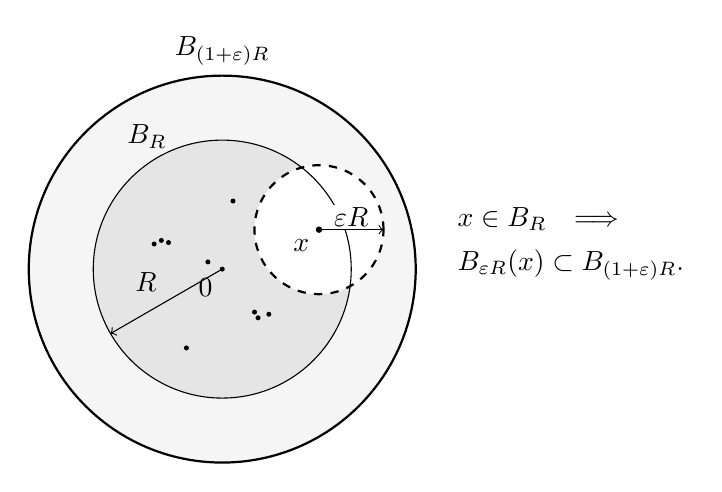
\begin{tikzpicture}[scale=.91]
 \fill[black!4] (0,0) circle (2.7);
 \fill[black!10] (0,0) circle (1.8);
 \fill[white] (1.35,.55) circle (.9);
 \draw[thick] (0,0) circle (2.7);
 \draw (0,0) circle (1.8);
 \draw[dashed,thick] (1.35,.55) circle (.9);
 \foreach \p in {(-.95,.35),(-.85,.4),(-.75,.37),(-.5,-1.1),
                  (.15,.95),(.45,-.6),(.5,-.68),(.65,-.63),(-.2,.1)}
   \fill \p circle (.035);
 \fill (0,0) circle (.035) node[below left] {$0$};
 \fill (1.35,.55) circle (.045) node[below left] {$x$};
 \draw[->] (0,0)--(-1.56,-.9)
   node[midway,above left] {$R$};
 \draw[->] (1.35,.55)--(2.25,.55)
   node[midway,above,fill=white,inner sep=1pt] {$\varepsilon R$};
 \node at (0,3.04) {$B_{(1+\varepsilon)R}$};
 \node at (-1.05,1.85) {$B_R$};
 \node[align=left,anchor=west] at (3.15,.35)
   {$x\in B_R$\quad$\Longrightarrow$\\[4pt]
    $B_{\varepsilon R}(x)\subset B_{(1+\varepsilon)R}$.};
\end{tikzpicture}
\caption{The comparison disk contains a disk of radius $\varepsilon R$
 around every $x\in\mathcal C_R$.  This containment gives the uniform tail
 error in \eqref{eq:uniform-cross-term}, including for clustered points.}
\label{fig:larger-disk}
\end{figure}

\Needspace{12\baselineskip}
The area self-term has the limit
\[
 \frac{Q(\nu_R,\nu_R)}{V_R}
 =\int_{\R^2}f(z)
   \frac{|B_{(1+\varepsilon)R}\cap(B_{(1+\varepsilon)R}-z)|}{V_R}
   \,\dd z
 \longrightarrow a.
\]
For each fixed $z$, the overlap fraction tends to one and is between zero
and one.  Dominated convergence therefore applies with dominator $|f|$.
In particular, $Q(\nu_R,\nu_R)>0$ for all sufficiently large $R$.
Cauchy--Schwarz and \eqref{eq:uniform-cross-term} now yield
\[
 \frac{Q(\mu_R,\mu_R)}{N_R}
 \ge\frac{|Q(\mu_R,\nu_R)|^2}{N_RQ(\nu_R,\nu_R)}
 =\frac{N_R}{V_R}\frac{(a+o(1))^2}{a+o(1)}.
\]
Since $N_R/V_R\to(1+\varepsilon)^{-2}$, taking the lower limit in $R$
and then letting $\varepsilon\downarrow0$ proves
\[
 \liminf_{R\to\infty}\frac{Q(\mu_R,\mu_R)}{N_R}\ge a.
\]
There are exactly $N_R$ diagonal terms, each equal to $f(0)$, so removing
them proves \eqref{eq:density-lp}.  The assertion for $\Phi$ follows by
termwise comparison of each finite off-diagonal sum.
\end{proof}

\FloatBarrier

\subsection{Sharp pairs for every Gaussian parameter}

The normalized theorem directly covers $\alpha\ge1$.
Fourier complementation supplies $0<\alpha<1$.  This is the Gaussian form
of the duality in Cohn and Miller~\citep[Section~6]{CohnMiller2016}; we give the calculation
to fix the dimension-two factor and the two contact sets.

\begin{lemma}[Gaussian duality]\label{lem:gaussian-duality}
For every $\alpha>0$, let $G_\alpha(x)=e^{-\pi\alpha|x|^2}$.
There is a real radial Schwartz function $f_\alpha$ such that, pointwise,
\begin{equation}\label{eq:gaussian-sharp-pair}
 \begin{gathered}
 f_\alpha\le G_\alpha,\qquad \widehat f_\alpha\ge0,\\
 f_\alpha(a)=G_\alpha(a)\quad(a\in A\setminus\{0\}),\qquad
 \widehat f_\alpha(w)=0\quad(w\in A^*\setminus\{0\}).
 \end{gathered}
\end{equation}
\end{lemma}

\begin{proof}
For $\alpha\ge1$, take
\[
 k=\pi(\alpha/b-h)\ge\pi(2/\sqrt3-2/5)>2.36.
\]
The elementary comparison is proved in Appendix~\ref{sec:arithmetic}.
Let $f$ be the function supplied by Theorem~\ref{thm:normalized-pair}
for this $k$, and define $f_\alpha=ke^{-k}f$.  The multiplier is positive,
so $\widehat f_\alpha\ge0$.  With $s=b|x|^2$, the upper bound for
$f_\alpha$ becomes
\[
 ke^{-k}e^{-\pi hs}T_k(s)
 =e^{-(\pi h+k)s}=e^{-\pi\alpha|x|^2}.
\]
The shell containment and $A^*=JA$ from Section~\ref{sec:fourier} place every
nonzero direct and dual shell in $\mathcal N$.  The value contacts in
\eqref{eq:normalized-jets} therefore give \eqref{eq:gaussian-sharp-pair}.

For $0<\alpha<1$, put $\beta=1/\alpha$ and use the function already
constructed for $\beta>1$.  Define its nonnegative radial Schwartz slacks
\[
 q_\beta=G_\beta-f_\beta,\qquad r_\beta=\widehat f_\beta.
\]
The Fourier transform applied twice is reflection, which is immaterial for
these radial functions.  Thus $G_\beta=q_\beta+\widehat r_\beta$.
The dimension-two Gaussian transform from
\eqref{eq:complex-gaussian-transform} gives
\[
 \beta^{-1}G_\alpha=\widehat G_\beta
 =\widehat q_\beta+r_\beta.
\]
Set
\begin{equation}\label{eq:reciprocal-minorant}
 f_\alpha=\beta\widehat q_\beta.
\end{equation}
Then $G_\alpha-f_\alpha=\beta r_\beta\ge0$ and
$\widehat f_\alpha=\beta q_\beta\ge0$.  The known contacts say that
$q_\beta$ vanishes on $A\setminus\{0\}$ and $r_\beta$ vanishes on
$A^*\setminus\{0\}$.  Since $A^*$ is a rotation of $A$ and both functions
are radial, $q_\beta$ also vanishes on the nonzero dual shells and
$r_\beta$ on the nonzero direct shells.  The two displayed slack identities
give the required contacts for $f_\alpha$.
\end{proof}

It remains to identify the lower bound with the Gaussian lattice sum.
Periodize the fixed Schwartz function $f_\alpha$ over $A$.  Schwartz decay
makes the periodization smooth, and termwise integration over a unit-area
fundamental cell gives Fourier coefficients $\widehat f_\alpha(w)$ for
$w\in A^*$.  These coefficients are absolutely summable.  Evaluating the
Fourier series at zero gives
$\sum_{a\in A}f_\alpha(a)=\sum_{w\in A^*}\widehat f_\alpha(w)$.
Using \eqref{eq:gaussian-sharp-pair} and removing the origin yields
\begin{equation}\label{eq:gaussian-lattice-value}
 \sum_{a\in A\setminus\{0\}}G_\alpha(a)
 =\widehat f_\alpha(0)-f_\alpha(0).
\end{equation}
Only the lattice has been periodized; no periodicity is assumed of the
competitor.  Proposition~\ref{prop:density-lp} with $\Phi=G_\alpha$ therefore
proves, for every locally finite $\mathcal C$ of centered disk density one
and every $\alpha>0$,
\begin{equation}\label{eq:gaussian-energy}
 \liminf_{R\to\infty}\frac1{N_R}
 \sum_{\substack{x,y\in\mathcal C_R\\x\ne y}}
 e^{-\pi\alpha|x-y|^2}
 \ge\sum_{a\in A\setminus\{0\}}e^{-\pi\alpha|a|^2}.
\end{equation}
This scalar inequality is the input for the positive-mixture argument in the
next section.  No measurable choice of the functions $f_\alpha$ will be
needed there.
